\chapter{Chapter 5: Memory Management}\label{ch-memory-management}

\section{Introduction}\label{introduction}

It's well-known to us right now that one of most important aspects in
modern operating systems is protecting the memory in a way that doesn't
allow a process to access or write to the memory of another process,
furthermore, the memory of the kernel should be protected from the
running processes, that is, they should be prevented from accessing
directly the memory of the kernel or writing to the memory of the
kernel. When we use the term \emph{memory of the kernel} or \emph{memory
of the process}, we mean the region of the main memory that is being
used by the kernel or the process and all of its data or code is stored
in this region of the memory.

In chapter \ref{ch-x86}, we have presented the distinction between the
logical view and physical view of the memory and one of the logical
views of the memory has been presented on the same chapter, this logical
view was segmented-memory model. We have seen how the hardware has
employed the protection techniques to provide memory protection and
protect the segments from each other. In the same chapter, we have
presented another logical view of the memory, it is flat-memory model,
which is exactly same as the physical view of the memory. In this view,
the memory is a big bunch of contiguous bytes and each byte has its
unique address that can be used to refer to this byte in order to read
it or to write to it.

We know that modern operating systems use the flat-memory model and
based on that we decided to use this model on 539kernel instead of the
segmented-memory model. Deciding which model to use is the job of the
kernelist. However, unlike segmentation, when we introduced the
flat-memory model, we haven't shown how the memory can be protected in
it, in this chapter we present one of the methods that can be used to
implement memory protection in flat-memory model. This technique is
known as \emph{paging}, it is a well-known technique that is used widely
by modern operating systems and it has a hardware support in x86
architecture.

\section{Paging in Theory}\label{paging-in-theory}

In paging, the memory of the process (before being loaded to the
physical memory) is divided into a number of fixed size blocks known as
\emph{pages}, in the same manner, the physical memory is divided into
blocks with the same fixed size, these blocks of physical memory are
known as \emph{page frames}. Figure \ref{fig:28092021_0} shows an
example of pages and page frames, as you can see in the figure, process
\lstinline!A! is divided into \lstinline!n! pages and the main memory is
divided into \lstinline!n! page frames, please note that the both
\lstinline!n!s shouldn't necessarily be equal. Because both page and
page frame have the same size, for example \lstinline!4KB! \footnote{That
  is, each page is of size \lstinline!4KB! and each page frame is of
  size \lstinline!4KB!,}, each page can be loaded exactly into one page
frame. To load process \lstinline!A! into the memory, each of its pages
should be loaded into a page frame. A page can be loaded into any page
frame, for example, let's assume we are loading page \lstinline!0! of
process \lstinline!A! and the first free page frame that we found is
page frame \lstinline!30!, then, the page \lstinline!0! can be loaded
into page frame \lstinline!30!. Of course, the pages of more than one
process can be loaded into the page frames.

\begin{figure}
\centering
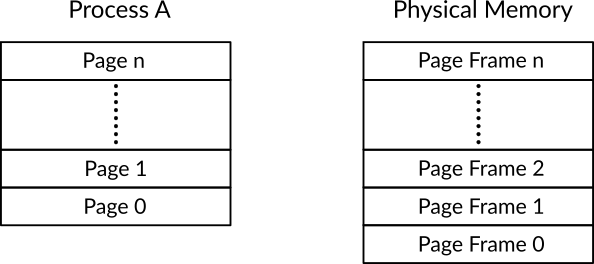
\includegraphics[width=0.35000\textwidth]{Figures/memory-ch/Fig28092021_0.png}
\caption{An Example that Shows Pages and Page
Frames}\label{fig:28092021_0}
\end{figure}

A data structure known as \emph{page table} is used to maintain these
information about the mapping between pages and their corresponding page
frame. Each process has its own page table, in our example of process
\lstinline!A!, the information that tells the processor that page
\lstinline!0! can be found in page frame \lstinline!30! is stored in
process \lstinline!A!'s page table. In paging, any memory address
generated by the process to read or write some data to the memory will
be a logical memory address \footnote{In x86, this logical memory
  address is known as \emph{linear memory address} as we have discussed
  earlier in chapter \ref{ch-x86}.}, that is, a not real not physical
memory address, it has a meaning for the process itself, but for the
processor it should be translated to the corresponding physical memory
address. The page table of the process is used to perform this
translation.

Basically, every generated logical memory address of a process running
in a paging-enabled environment is composed of the following parts: the
page number and the offset. For example, assume a system which employs
paging with length of \lstinline!2! bytes for memory addresses
\footnote{In 32-bit x86 architecture, the length of memory address is
  \lstinline!4 bytes = 32 bits!, that is, \lstinline!2^32 bytes = 4GB!
  are addressable. An example of a memory address in this environment is
  \lstinline!FFFFFFFFh! which is of length \lstinline!4 bytes! and
  refers to the last byte of the memory.}. In this hypothetical system,
the format of logical address is the following, the first byte
represents the page number and the second byte represents the offset.
Process \lstinline!B! is a process that runs in that system, assume that
it performed an instruction to read data from the following memory
address \lstinline!0150h!, this is a logical memory address that needs
to be translated to the physical address to be able to get the required
content. Based on the format of the logical memory addresses in this
system, the first byte of the generated memory address which is
\lstinline!01h! represents the page, that means that the required data
is stored in page \lstinline!01h = 1d! of the process \lstinline!B!, but
where exactly? According the the generated address, it is on the offset
\lstinline!50h = 80d! of that page.

To perform the translation and get the physical memory address, we need
to know in which page frame the page \lstinline!1! of process
\lstinline!B! is loaded. To answer this question the page table of
process \lstinline!B! should be consulted. For each page, there is an
entry in the page table that contains necessary information, and of
course one of those information is the page frame that this page is
stored on. This information can be the page frame number or the base
memory address of the page frame, it doesn't matter since we can get the
base memory address of the page frame by knowing its number and the size
of page frames. After getting the base memory address, we can combine it
with the required offset to get the physical memory address of the data
in question. The hardware that is responsible for the process of memory
address translation is known as \emph{memory management unit} (MMU).

Sometimes, the page table is divided into more than one level. For
example, in two-level page table, the entries of the main page table
refers to an entry on another page table that contains the the base
address of the page frame, x86 architecture uses this design, so we are
going to see it on details later on. The reason of using such design is
the large size of page tables for a large main memory. As you know, the
page table is a data structure that should reside in the main memory
itself, and for each page there is an entry in the page table, in x86
for example, the size of this entry is \lstinline!8! bytes. Furthermore,
the size a page tend to be small, \lstinline!4KB! is a real example of
page size. So, if \lstinline!4GB! is needed to be represented by a page
table with \lstinline!8! bytes of entry size, then \lstinline!8MB! is
needed for this page table which is not a small size for a data
structure needed for each process in the system.

It should be clear by now how paging provides memory protection. Any
memory address that is generated by the process will be translated to
the physical memory by the hardware, there is no way for the process to
access the data of any other process since it knows nothing about the
physical memory and how to reach it. Consider process \lstinline!C! that
runs on the same hypothetical system that we have described above, in
the memory location that's represented by the physical memory address
\lstinline!A1 9Bh! there is some important data which is stored by the
kernel and process \lstinline!C! wishes to read it. If process
\lstinline!C! tries the normal way to read from the memory address
\lstinline!A1 9Bh! the \lstinline!MMU! of the system is going to
consider it as a logical memory address, so, the page table of process
\lstinline!C! is used to identify in which page frame that page
\lstinline!00A1h! of process \lstinline!C! is stored. As you can see,
the process knows nothing about the outside world and cannot gain this
knowledge, it thinks it is the only process in the memory, and any
memory address it generates belongs to itself and it cannot interfere
the translation process or modify its own page table.

\section{Virtual Memory}\label{virtual-memory}

In multitasking system, beside the need of memory protection, also, the
main memory should be utilized as much as we can. In such environment,
multiple processes should reside in the main memory and at some point of
time the main memory will become full and the kernel will not be able to
create any new process before stopping a currently running process to
use its space in the main memory.

There are many situations where the current processes are occupying a
space from the main memory but doesn't really use this space, that
wastes this space since it can be used to load a process that really
needs this space. An example of these situations is when the process is
idle, that is, doing nothing but waiting for some external action
(e.g.~a button click), in this case the only active code of this process
that should be in the main memory is the code that makes the process
waits for an event. Furthermore, modern software tend to be too large,
there are a lot of routines in a code of modern software that might not
be called at all during executing that software, loading the code of
those routines into the main memory wastes the occupied space, the
routines will be there in the memory, taking some space that can be used
for more useful purposes and they will never be called.

Virtual memory is a memory management technique that can be used to
utilize the main memory. You might noticed in modern operating systems,
you can open any number of software in a given time and you never get a
message from the operating system that tells you that there is no enough
space in the main memory although the software that you are running need
a large space of memory (modern web browsers are obvious example), how
can that be achieved? Well, by using virtual memory which depends on
paging that we have discussed earlier.

Regarding to paging, we may ask ourselves an important question, should
all process' pages be loaded into the memory? In fact, not really. As we
have said, the binary code of the software may have a lot of routines
that may not be called, so, the pages that contain these routines should
not be loaded into the memory since they will not be used, instead, this
space can be used for another pages that should really be on the memory.
To realize that, when the software is loaded for the first time, only
the page the contains the entry code of the software (e.g.
\lstinline!main! function in C) is loaded into the memory, not any other
page of that software. When some instruction in the entry code tries to
read data or call a routine that doesn't exist on the loaded page, then,
the needed page will be loaded into the main memory and that piece which
was not there can be used after this loading, that is, any page of the
process will not be loaded into a free page frame unless it's really
needed, otherwise, it will be waiting on the disk, this is known as
\emph{demand paging}.

By employing demand paging, virtual memory saves a lot of memory space.
Furthermore, virtual memory uses the disk for two things, first, to
store the pages that are no demanded yet, they should be there so
anytime one of them is needed, it can be loaded from the disk to the
main memory. Second, the disk is used to implement an operation known as
\emph{swapping}.

Even with demand paging, at some point of time, the main memory will
become full, in this situation, when a page is needed to be loaded the
kernel that implements virtual memory should load it, even if the memory
is full! How? The answer is by using the swapping operation, one of page
frames should be chosen to be removed from the main memory, this frame
in this case is known as \emph{victim frame}, the content of this frame
is written into the disk, it is being \emph{swapped out}, and its place
in the main memory is used for the new page that should be loaded. The
swapped out page is not in the main memory anymore, so, when it is
needed again, it should be reloaded from the disk to the main memory.

The problem of which victim frame should be chosen is known as
\emph{page replacement} problem, that is, when there is no free page
frame and a new page should be loaded, which page frame should we make
free to be able to load the new page. Of course, there are many page
replacement algorithms out there, one of them is \emph{first-in
first-out} in which the page frame that was the first one to be loaded
among the current page frames is chosen as a victim frame. Another
well-known algorithm is \emph{least recently used} (LRU), in this
algorithm, everytime the page is accessed, the time of access is stored,
when a victim frame is needed, then it will be the oldest one that has
been accessed.

The page table can be used to store a bunch of information that are
useful for virtual memory. First, a page table usually has a flag known
as \emph{present}, by using this flag, the processor can tell if the
page that the process tries to access is loaded into the memory or not,
if it is loaded, then a normal access operation is performed, but when
the present flag indicates that this page is not in the memory, what
should be done? For sure, the page should be loaded from the disk to the
memory. Usually, the processor itself doesn't perform this loading
operation, instead, it generates an exception known as \emph{page fault}
and makes the kernel deal with it. A page fault tells the kernel that
one of the processes tried to access a not-loaded page, so it needs to
be loaded. As you can see, page faults help in implementing demand
paging, anytime a page needs to be loaded into the memory then a page
fault will be generated.

With this mechanism that virtual memory uses to manage the memory, we
can make a process to own a size of memory that is not even available on
the system. For example, in x86 architecture with systems that employ
virtual memory, each process thinks that it owns \lstinline!4GB! of main
memory, even if the system has only \lstinline!2GB! of RAM for instance.
This is possible due to demand paging and page replacements. Of course,
a large size of memory being available for the process, makes it easier
for the programmers to write their code.

\section{Paging in x86}\label{paging-in-x86}

In x86, unlike segmentation which is enabled by default, paging is
disabled by default, also, paging is not available on real mode, in
\lstinline!32-bit! environment it can only be used in protected-mode
\footnote{In 64-bit architecture paging is available in both
  protected-mode and long-mode.}. If paging is intended to be used, the
kernel should switch to protected-mode first, then, enables paging
through a special register in x86 known as \lstinline!CR0! which is one
of \emph{control registers} of x86 architecture. The last bit of
\lstinline!CR0! is the one that decides if paging is enabled, when its
value is \lstinline!1!, or disabled when its value is \lstinline!0!.

There are three \emph{paging modes} in x86 a kernelist can chooses from,
the difference between these three modes is basically related to the
size of memory addresses and the available sizes of a page. These modes
are \emph{32-bit paging}, \emph{PAE paging} (PAE stands for ``Physical
Address Extension'') and \emph{4-level paging} which is available for
\lstinline!64-bit! environment only.

Beside the last bit in \lstinline!CR0!, there are another two bits that
can be used to decide the current paging mode. The first one is known as
\emph{PAE bit} which is the fifth bit of the control register
\lstinline!CR4!. When the value of this bit is \lstinline!1! that means
PEA mode is enabled, while \lstinline!0! means otherwise. The second bit
is known as \lstinline!LME! in a register known as
\lstinline!IA32_EFER!, setting the value of this register to
\lstinline!1! makes the processor to switch from the protected-mode
(\lstinline!32-bit! environment) to the long-mode (\lstinline!64-bit!
environment) and when the value of \lstinline!PAE! bit is \lstinline!1!,
then 4-level mode will be enabled.

In our next discussions, we are going to focus on \lstinline!32-bit!
paging mode which is the most basic one that is available for
\lstinline!32-bit! environment. In this mode, there are two available
sizes for a page \lstinline!4KB! and \lstinline!4MB!, also,
\lstinline!4GB! of memory is addressable in this mode.

\subsection{The Structure of Linear Memory
Address}\label{the-structure-of-linear-memory-address}

Previously, we have discussed a part of the translation process of
memory addresses in x86. To sum what we have already discussed up, any
memory address that is generated by an executing code in x86 is known as
a logical address, which is not the real memory address that contains
the required data. This logical address need to be translated to get the
real address. The first step of this translation process is to use
segment descriptors to translate a logical address to a linear address
by using the mechanism that we have already mentioned in chapter
\ref{ch-x86}. When paging is disabled, the resulted linear address will
be the physical (real) address that can be sent to the main memory to
get the required data. On the other hand, when paging is enabled, the
linear address needs a further translation step to obtain the physical
memory address by using paging mechanism. To be able to perform this
step of translation, a page table is used with the parts that compose
the linear address.

\begin{figure}
\centering
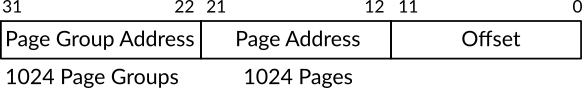
\includegraphics[width=0.35000\textwidth]{Figures/memory-ch/Fig091021_0.png}
\caption{The Structure of Linear Address}\label{fig:10062021_3}
\end{figure}

Figure \ref{fig:10062021_3} shows the structure of a linear address and
its parts. As you can see, the size of a linear address is
\lstinline!32-bit! which is divided into three parts. The bits
\lstinline!22! to \lstinline!31! represent a \emph{page directory}
entry, the bits \lstinline!12! to \lstinline!21! represent a page table
entry and the bits \lstinline!0! to \lstinline!11! represent an offset
that contains the required data within a page frame. For example, assume
a linear address which is composed of the following: page directory
entry \lstinline!x!, page table entry \lstinline!y! and offset
\lstinline!z!. That means that this linear address needs to read the
offset \lstinline!z! from a page that is represented by the entry
\lstinline!y! in the page table, and this page table is represented by
the page directory entry \lstinline!x!.

As you can see here, unlike our previous discussion of page table, the
one which is implemented in x86 is a two-level page table, the first
level is known as \emph{page directory} which is used to point to the
second level which is a page table and each page table, as we know,
points to a page frame. As we mentioned before, the reason of using
multi-level page tables is to save some memory since the size of page
tables tend to have relatively large sizes in modern architecture and
given that each process needs its own page table, then, its better to
use multi-level page table which allows us to load just the needed parts
of a page table (in a way similar to paging) instead of loading the
whole page table into the memory.

\subsection{Page Directory}\label{page-directory}

The page directory in x86 can hold up to \lstinline!1024! entries. Each
entry points to a page table and each one of those page tables can hold
up to \lstinline!1024! entries which represent a process's pages. In
other words, we can say that, for each process, there are more than one
page table, and each one of those page tables is loaded in a different
part of the main memory and the page directory of the process helps us
in locating the page tables of a process.

As we have mentioned before, the page directory is the first level of
x86's page table and each process has its own page directory. How the
processor can find the current page directory, that is, the page
directory of the current process? This can be done by using the register
\lstinline!CR3! which stores the base physical memory address of the
current page directory. The first part of a linear address is an offset
within the page directory, when an addition operation is performed
between the first part of a linear address and the value on
\lstinline!CR3! the result will be the base memory address of the entry
that represents a page table that contains an entry which represents the
page that contains the required data.

\subsubsection{The Structure of a Page Directory
Entry}\label{the-structure-of-a-page-directory-entry}

The size of an entry in the page directory is \lstinline!4! bytes
(\lstinline!32! bits) and its structure is shown in the figure
\ref{fig:10102021_0}. The bits from \lstinline!12! to \lstinline!31!
contain the physical memory address of the page table that this entry
represent. Not all page tables that a page directory points to should be
loaded into the main memory, instead, only the needed page tables, the
rest are stored in a secondary storage until they are needed then they
should be loaded. To be able to implement this mechanism, we need some
place to store a flag that tells us whether the page table in question
is loaded into the main memory or not, and that's exactly the job of bit
\lstinline!0! of a page directory entry, this bit is known as
\emph{present bit}, when its value is \lstinline!1! that means the page
table exists in the main memory, while the value \lstinline!0! means
otherwise. When an executing code tries to read a content from a page
frame that its page table is not in the memory, the processor generates
a page fault that tells the kernel to load this page table because it is
needed right now.

\begin{figure}
\centering
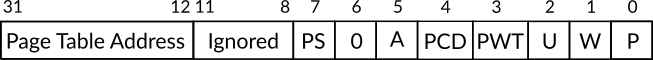
\includegraphics[width=0.35000\textwidth]{Figures/memory-ch/Fig10102021_0.png}
\caption{The Structure of Page Directory Entry}\label{fig:10102021_0}
\end{figure}

When we have discussed segment descriptors, we have witnessed some bits
that aim to provide additional protection for a segment. Paging in x86
also has bits that help in providing additional protection. Bit
\lstinline!1! in a page directory entry decides whether the page table
that the entry points to is read-only when its value is \lstinline!0! or
if its writable \lstinline!1!. Bit \lstinline!2! decides whether the
access to the page table that this entry points to is restricted to
privileged code, that is, the code that runs on privilege level
\lstinline!0!, \lstinline!1! and \lstinline!2! when the bit's value is
\lstinline!0! or that the page table is also accessible by a
non-privileged code, that is, the code that runs on privilege level
\lstinline!3!.

Generally in computing, \emph{caching} is a well-known technique. When
caching is employed in a system, some data are fetched from a source and
stored in a place which is faster to reach if compared to the source,
these stored data are known as \emph{cache}. The goal of caching is to
make a frequently accessed data faster to obtain. Think of your web
browser as an example of caching, when use visit a page \footnote{Please
  do not confuse a web page with a process page in this example.} in a
website, the web browser fetches the images of that page from the source
(the server of the website) and stores it in your own machine's storage
device which is definitely too much faster to access if compared to a
web server, when you visit the same website later, and the web browser
encounters an image to be shown, it searches if it's cached, if so, this
is known as \emph{cache hit}, the image will be obtained from your
storage device instead of the web server, if the image is not cached,
this is known as \emph{cache miss}, the image will be obtained from the
web server to be shown and cached.

The processor is not an exception, it also uses cache to make things
faster. As you may noticed, the entries of page directories and page
tables are frequently accessed, in the code of software a lot of memory
accesses happen and with each memory access both page directory and
pages tables need to be accessed. With this huge number of accesses to
page table and given the fact that the main memory is too much slower
than the processor, then some caching is needed, and that exactly what
is done in x86, a part of the page directory and page tables are cached
in an internal, small and fast memory inside the processor known as
\emph{translation lookaside buffer} (\lstinline!TLB!), each time an
entry of page table of directory is needed, this memory is checked
first, if the needed entry is on it, that is, we got a cache hit, then
it will be used.

In x86 paging, caching is controllable, say that for some reason, you
wish to disable caching for a given entry, that can be done with bit
\lstinline!4! in a page directory entry. When the value of this bit is
\lstinline!1!, then the page table that is represented by this entry
will not be cached by the processor, but the value \lstinline!0! in this
bit means otherwise.

Unlike web browsers, the cached version of page table can be written to,
for example, assume that page table \lstinline!x! has been cached after
using it in the first time and there is a page in this page table, call
it \lstinline!y!, that isn't loaded into the memory. We decided to load
the page \lstinline!y! which means present bit of the entry that
represents this page should be changed in the page table \lstinline!x!.
To make things faster, instead of writing the changes to the page table
\lstinline!x! in the main memory (the source), these changes will be
written to the cache which makes a difference between the cached data
and the source data, that is, they are not identical anymore. This
inconsistency between the two places that store the data should be
resolved somehow, the obvious thing to do is to write these changes
later also on the source.

In caching context, the timing of writing the changes to the source is
known as \emph{write policy} and there are two available policies in x86
for page tables and directory caches, the first one is known as
\emph{write-through}, in this policy, the new data is written on both
the cache and the source at same time. The second policy is known as
\emph{write-back}, in which the writing process is performed only on the
cache, while writing the changes on the source is performed later, for
example when we decide to clear the cache. Bit \lstinline!3! of the page
directory entry decides which write policy will be used for the cached
data, the value \lstinline!1! means write-through policy will be used,
while the value \lstinline!0! means write-back policy will be used.

As in segment descriptors, when a page table which is referred by a
given page directory entry is accessed, there is a bit in the directory
entry known as \emph{access bit} which is the fifth bit in the entry.
The processor sets the value \lstinline!1! automatically when the page
table is accessed. Setting the value to \lstinline!0! for any reason is
the responsibility of the kernel.

We have said earlier that \lstinline!32-bit! paging in x86 provides us
with two possible options for the size of a page, either \lstinline!4KB!
page or \lstinline!4MB! page. The bit \lstinline!7! in a page directory
entry decides the size of the pages, when its value is \lstinline!0!
then the page size will be \lstinline!4KB! while the value \lstinline!1!
means that the page size is \lstinline!4MB!. There is a major difference
between the two options. When the size of the page is \lstinline!4MB!,
the page table will be a normal one-level page table, which means that
the page directory will not refer to a page table anymore, but it is
going to refer to a page frame. When the size of the page is
\lstinline!4KB!, the two-level hierarchy will be employed. That makes
sense, the number of entries that are needed to represent
\lstinline!4KB! pages are way more than the number of entries that are
needed to represent \lstinline!4MB! pages. However, in our discussion,
we have focused (and will focus) on the case of \lstinline!4KB! pages.
Finally, the bits \lstinline!6!, \lstinline!8!, \lstinline!9!,
\lstinline!10! and\lstinline!11! in the page directory entry are
ignored.

\subsection{Page Table}\label{page-table}

In \lstinline!4KB! pages environment, a page table is referred to by an
entry in the page directory. As mentioned earlier, each page table can
hold \lstinline!1024! entries. After finding the base memory address of
the page table in question by consulting the page directory, this base
memory address will be used with the second part of the linear address
to figure out which page table entry should the processor consult to
reach the required data in the physical memory. Of course, the most
important information that a page table entry stores is the base
physical memory address of the page frame, this memory address will be
used with the third part of the linear address (offset) to get the final
physical memory address.

The entry of a page table is exactly same as the entry of a page
directory, its size is \lstinline!4! bytes. Though, there are some
simple differences, the first difference is bit \lstinline!7!, which was
used to decide the page size in page directory, is ignored in the entry
of a page table. The second difference is in bit \lstinline!6!, which
was ignored in the entry of page directory, in page tables this bit is
known as \emph{dirty bit}.

In our previous discussion on virtual memory we know that at some point
of time, a victim frame may be chosen. This frame is removed from the
main memory to free up some space for another page that we need to load
from the disk. When the victim frame is removed from the main memory,
its content should be written to the disk since its content may have
been changed while it was loaded into the memory. Writing the content of
the victim frame to the disk and loading the new page also from disk,
given that the disk is really too slow compared to the processor, is
going to cause some performance penalty.

To make the matter a little bit better, we should write the content of
the victim frame only if there is a real change in its content compared
to the version which is already stored in the disk. If the victim frame
version which is on the main memory and the version on the disk are
identical, there is no need to waste valuable resource on writing the
same content on the disk, for example, page frames that contain only
code will most probably be the same all the time, so their versions on
disk and main memory will be identical. The dirty bit is used to
indicate whether the content of the page frame has been changed and has
differences with the disk version, that is, the page (when the value of
the bit \lstinline!1!) or the two versions are identical (value
\lstinline!0!).

\section{Paging and Dynamic Memory in
539kernel}\label{paging-and-dynamic-memory-in-539kernel}

The last result of this section is version \lstinline!G! of 539kernel
which contains the basic stuff that are related to the memory.
Previously, we have seen that we have no way in 539kernel to allocate
memory dynamically, due to that, the allocation of entries of processes
table and the process control block was a static allocation. Making
dynamic allocation possible is an important thing since a lot of
kernel's objects need to be allocated dynamically. Therefore, the first
memory-related thing to implement is a way to allocate memory
dynamically. The other major part of version \lstinline!G! is
implementing paging by using x86 architecture's support. Since there is
no way yet in 539kernel to access the hard disk, virtual memory cannot
be implemented yet. However, basic paging can be implemented and this
can be used as basis for further development.

\subsection{Dynamic Memory Allocation}\label{dynamic-memory-allocation}

As we have mentioned earlier, in our normal process of developing
applications by using programming languages that don't employ garbage
collection, we are responsible for allocating spaces from memory. When
we need to store data in memory, a free space in memory should be
available for this data to put this data in. The process of telling that
we need \lstinline!n! bytes from memory to store some data is known as
memory allocation. There are two possible ways to allocate memory,
statically or dynamically.

Usually, a static memory allocation is used when we know the size of
data at compile time, that is, before running the application that we
are developing. Dynamic memory allocation is used when the size of data
will be known at run time. Static memory allocation is the
responsibility of the compiler of the language that we are using, while
the dynamic memory allocation is the responsibility of the programmer
\footnote{Not in all cases though.}, also, the regions that we have
allocated dynamically should be freed manually \footnote{This holds true
  in the case of programming languages like C. New system programming
  languages such as Rust for example may have different ways to deal
  with the matter. However, what we are discussing here is the basis,
  depending on this basis more sophisticated concepts (e.g.~Rust) can be
  built.}.

As we have seen, there are multiple region of a running process's memory
and each region has a different purpose, we already discussed run-time
stack which is one of those region. The other data region of a process
that we also discussed previously is the run-time heap. When we allocate
memory dynamically, the memory region that we have allocated is a part
of the run-time heap, which is a large region of process memory that is
used for dynamic allocation, in C, for example, the most well-known way
to allocate bytes dynamically, that is, from the run-time heap is to use
the function \lstinline!malloc! which implements an algorithm known as
\emph{memory allocator}. The run-time heap need to be managed, due to
that, this kind of algorithms use data structures that maintain
information about the allocated space and free space.

A need of dynamic memory allocation have shown up previously in
539kernel. Therefore, in the current version 539kernel we are going to
implement the most basic memory allocator possible. Through a new
function \lstinline!kalloc! (short for \emph{kernel allocate}), which
works in a similar way as \lstinline!malloc!, a bunch of bytes can be
allocate from the kernel's run-time heap, the starting memory address of
this allocated region will be returned by the function, after that, the
region can be used to store whatever we wish. The stuff that are related
to the kernel's run-time heap will be defined in a new file
\lstinline!heap.c! and its header file \lstinline!heap.h!, let's start
with the latter which is the following.

\begin{lstlisting}[language=C]
unsigned int heap_base;

void heap_init();
int kalloc( int );
\end{lstlisting}

A global variable known as \lstinline!heap_base! is defined, this
variable contains the memory address that the kernel's run-time heap
starts from, and starting from this memory address we can allocate
user's needed bytes through the function \lstinline!kalloc! which its
prototype is presented here.

As usual, with each subsystem in 539kernel, there is an initialization
function that sets the proper values and does whatever needed to make
this subsystem ready to use, as you may recall, these functions are
called right after the kernel starts in protected mode, in our current
case \lstinline!heap_init! is the initialization function of the
kernel's run-time heap. We can now start with \lstinline!heap.c!, of
course, the header file \lstinline!heap.h! is needed to be included in
\lstinline!heap.c!, and we begin with the code of \lstinline!heap_init!.

\begin{lstlisting}[language=C]
#include "heap.h"

void heap_init()
{
    heap_base = 0x100000;
}
\end{lstlisting}

As you can see, the function \lstinline!heap_init! is too simple. It
sets the value \lstinline!0x100000! to the global variable
\lstinline!heap_base!. That means that kernel's run-time heap starts
from the memory address \lstinline!0x100000!. In \lstinline!main.c! we
need to call this function in the beginning to make sure that dynamic
memory allocation is ready and usable by any other subsystem, so, we
first add \lstinline!#include "heap.h"! in including section of
\lstinline!main.c!, then we add the call line \lstinline!heap_init();!
in the beginning of \lstinline!kernel_main! function. Next is the code
of \lstinline!kalloc! in \lstinline!heap.c!.

\begin{lstlisting}[language=C]
int kalloc( int bytes )
{
    unsigned int new_object_address = heap_base;
    
    heap_base += bytes;
    
    return new_object_address;
}
\end{lstlisting}

Believe it or not! This is a working memory allocator that can be used
for dynamic memory allocation. It's too simple, though, it has some
disadvantages but in our case it is more than enough. It receives the
number of bytes that the caller needs to allocate from the memory
through a parameter called \lstinline!bytes!.

In the first step of \lstinline!kalloc!, the value of
\lstinline!heap_base! is copied to a local variable named
\lstinline!new_object_address! which represents the starting memory
address of newly allocated bytes, this value will be returned to the
caller so the latter can start to use the allocated memory region
starting from this memory address.

The second step of \lstinline!kalloc! adds the number of allocated bytes
to \lstinline!heap_base!, that means the next time \lstinline!kalloc! is
called, it starts with a new \lstinline!heap_base! that contains a
memory address which is right after the last byte of the memory region
that has been allocated in the previous call. For example, assume we
called \lstinline!kalloc! for the first time with \lstinline!4! as a
parameter, that is, we need to allocate four bytes from kernel's
run-time heap, the base memory address that will be returned is
\lstinline!0x100000!, and since we need to store four bytes, we are
going to store them on the memory address \lstinline!0x100000!,
\lstinline!0x100001!, \lstinline!0x100002! and \lstinline!0x100003!
respectively. Just before returning the base memory address,
\lstinline!kalloc! added \lstinline!4!, which is the number of required
bytes, to the base of the heap \lstinline!heap_base! which initially
contained the value \lstinline!0x100000!, the result is
\lstinline!0x100004! which will be stored in \lstinline!heap_base!. Next
time, when \lstinline!kalloc! is called, the base memory address of the
allocated region will be \lstinline!0x100004! which is, obviously, right
after \lstinline!0x100003!.

As you can see from the allocator's code, there is no way to implement
\lstinline!free! function, usually, this function takes a base memory
address of a region in run-time heap and tells the memory allocator that
the region which starts with this base address is free now and can be
used for other allocations. Freeing memory regions when the code
finishes from using them helps in ensuring that the run-time heap is not
filled too soon, when an application doesn't free up the memory regions
that are not needed anymore, it causes a problem known as \emph{memory
leak}.

In our current memory allocator, the function \lstinline!free! cannot be
implemented because there is no way to know how many bytes to free up
given the base address of a memory region, returning to the previous
example, the region of run-time heap which starts with the base address
\lstinline!0x100000! has the size of \lstinline!4! bytes, if we want to
tell the memory allocator to free this region, it must know what is the
size of this region which is requested to be freed, that of course means
that the memory allocator needs to maintain a data structure that can be
used at least when the user needs to free a region up, one simple way to
be able to implement \lstinline!free! in our current memory allocator is
to modify \lstinline!kalloc! and make it uses, for example, a
linked-list, whenever \lstinline!kalloc! is called to allocate a region,
a new entry is created and inserted into the linked-list, this entry can
be stored right after the newly allocated region and contains the base
address of the region and its size, after that, when the user request to
free up a region by giving its base memory address, the \lstinline!free!
function can search in this linked-list until it finds the entry of that
region and put on the same entry that this region is now free and can be
used for future allocation, that is, the memory which was allocated once
and freed by using \lstinline!free! function, can be used later somehow.

Our current focus is not on implementing a full memory allocator, so, it
is up to you as a kernelist to decide how your kernel's memory allocator
works, of course, there are a bunch of already exist algorithm as we
have mentioned earlier.

\subsubsection{Using The Allocator with Process Control
Block}\label{using-the-allocator-with-process-control-block}

To make sure that our memory allocator works fine, we can use it when a
new process control block is created. It also can be used for processes
table, as you may recall, the processes table from version \lstinline!T!
is an array which is allocated statically and its size is
\lstinline!15!, instead, the memory allocator can be used to implement a
linked-list to store the list of processes. However, for the sake of
simplicity, we will stick here with creating PCB dynamically as an
example of using \lstinline!kalloc!, while keeping the processes table
for you to decide if it should be a dynamic table or not and how to
design it if you decide that it should be dynamic.

The first thing we need to do in order to allocate PCBs dynamically is
to change the parameters list of the function \lstinline!process_create!
in both \lstinline!process.h! and \lstinline!process.c!. As you may
recall, in version \lstinline!T!, the second parameter of this function
called \lstinline!process! and it was the memory address that we will
store the PCB of the new process on it. We had to do that since dynamic
memory allocation wasn't available, so, we were creating local variables
in the caller for each new PCB, then we pass the memory address of the
local variable to \lstinline!process_create! to be used for the new PCB.
This second parameter is not needed anymore since the region of the new
PCB will be allocated dynamically by \lstinline!kalloc! and its memory
address will be returned by the same function. So, the prototype of the
function \lstinline!process_create! will be in \lstinline!process.h! and
\lstinline!process.c! respectively as the following.

\begin{lstlisting}[language=C]
process_t *process_create( int * );
\end{lstlisting}

\begin{lstlisting}[language=C]
process_t *process_create( int *base_address )
\end{lstlisting}

You can also notice that the function now returns a pointer to the newly
created PCB, in version \lstinline!T! it was returning nothing. The next
changes will be in the code of \lstinline!process_create!. The name of
the eliminated parameter of \lstinline!process_create! was
\lstinline!process! and it was a pointer to the type
\lstinline!process_t!. We substitute it with the following line which
should be in the beginning of \lstinline!process_create!.

\begin{lstlisting}[language=C]
process_t *process = kalloc( sizeof( process_t ) );
\end{lstlisting}

Simply, we used the same variable name \lstinline!process! but instead
of getting it as a parameter we define it as a local variable, we call
the memory allocator to allocate a region that has the same size of the
type \lstinline!process_t! from the kernel's run-time heap, exactly as
we do in user-space applications development, so, the new memory region
can be used to store the new PCB and its memory address is stored in the
local variable \lstinline!process!. In the last of
\lstinline!process_create! we should add the line
\lstinline!return process;! to return the memory address for the newly
created PCB for the new process.

In version \lstinline!T! we have called \lstinline!process_create! in
\lstinline!main.c! to create four processes, we need to change the calls
by omitting the second parameter, also the line
\lstinline!process_t p1, p2, p3, p4;! in \lstinline!main.c! which was
allocating memory for the PCBs can be removed since we don't need them
anymore. The calls of \lstinline!process_create! will be as the
following.

\begin{lstlisting}[language=C]
process_create( &processA );
process_create( &processB );
process_create( &processC );
process_create( &processD );
\end{lstlisting}

\subsection{Paging}\label{paging}

In this section we are going to implement a basic paging for 539kernel.
To do that, a number of steps should be performed. A valid page
directory should be initialized and its address should be loaded in the
register \lstinline!CR3!. Also, paging should be enabled by modifying
the value of \lstinline!CR0! to tell the processor to start using paging
and translate linear memory addresses by using the page tables instead
of consider those linear addresses as physical addresses. We have
mentioned earlier, for each process we should define a page table,
however, in this section we are going to define the page table of the
kernel itself since this is the minimum requirement to enable paging.

The page size in 539kernel will be \lstinline!4KB!, that means we need a
page directory that can point to any number of page tables up to
\lstinline!1024! page table. The mapping itself will be \emph{one-to-one
mapping}, that is, each linear address will be translated to a physical
address and both are identical. For example, in one-to-one mapping the
linear address \lstinline!0xA000! refers to the physical address
\lstinline!0xA000!. This choice has been made to make things simple,
more advanced designs can be used instead. We already know the concept
of page frame, when the page size is \lstinline!4KB! that means page
frame \lstinline!0! is the memory region that starts from the memory
address \lstinline!0! to \lstinline!4095d!. One-to-one mapping is
possible, we can simply define the first entry of the first page table
\footnote{The first page table is the one which is pointed to by the
  first entry in the page directory.} to point to page frame
\lstinline!0! and so on. The memory allocator will be used when
initializing the kernel's page directory and page tables, we can
allocate them statically as we have done with \lstinline!GDT! for
example, but that can increase the size of kernel's binary file.

Before getting started with the details two new files are needed to be
created: \lstinline!paging.h! and \lstinline!paging.c! which will
contain the stuff that are related to paging. The content of
\lstinline!paging.h! is the following.

\begin{lstlisting}[language=C]
#define PDE_NUM 3
#define PTE_NUM 1024

extern void load_page_directory();
extern void enable_paging();

unsigned int *page_directory;

void paging_init();
int create_page_entry( int, char, char, char, char, char, char, char, char );
\end{lstlisting}

The part \lstinline!PDE! in the name of the macro \lstinline!PDE_NUM!
means page directory entries, so this macro represents the number of the
entries that will be defined in the kernel's page directory. Any page
directory may hold \lstinline!1024! entries but in our case not all of
these entries are needed so only \lstinline!3! will be defined instead,
that means only three page tables will be defined for the kernel. How
many entries will be defined in those page tables is decided by the
macro \lstinline!PTE_NUM! which \lstinline!PTE! in its name means page
table entries, its value is \lstinline!1024! which means there will be
\lstinline!3! entries in the kernel's page directory and each one of
them points to a page table which has \lstinline!1024! entries. The
total entries will be \lstinline!3 * 1024 = 3072! and we know that each
of these entries map a page frame of the size \lstinline!4KB! then
\lstinline!12MB! of the physical memory will be mapped in the page table
that we are going to define, and since our mapping will be one-to-one,
that means the reachable physical memory addresses start at
\lstinline!0! and ends at \lstinline!12582912!, any region beyond this
range, based on our setting, will not be reachable by the kernel and it
is going to cause a page fault exception. It is your choice to set the
value of \lstinline!PDE_NUM! to the maximum (\lstinline!1024!), this
will make a \lstinline!4GB! of memory addressable.

Getting back to the details of \lstinline!paging.h!, both
\lstinline!load_page_directory! and \lstinline!enable_paging! are
external functions that will be defined in assembly and will be used in
\lstinline!paging.c!. The first function loads the address of the
kernel's page directory in the register \lstinline!CR3!, this address
can be found in the global variable \lstinline!page_directory! but of
course, its value will be available after allocating the needed space by
\lstinline!kalloc!. The second function is the one that modifies the
register \lstinline!CR0! to enable paging in x86, this should be called
after finishing the initialization of kernel's page directory and
loading it.

\subsubsection{Initializing Kernel's Page Directory and
Tables}\label{initializing-kernels-page-directory-and-tables}

From our previous encounter with the structure of page directory/table
entry, we know that the size of this entry is \lstinline!4! bytes and
has a specific arrangement of the bits to indicate the properties of the
entry being pointed to. The function \lstinline!create_page_entry! helps
in constructing a value that can be stored in a page directory/table
entry based on the properties that should be enabled and disabled, this
value will be returned to the caller. As you can see from
\lstinline!paging.h!, it returns an integer and that makes sense, as we
know, the size of integer in \lstinline!32-bit! architecture C is
\lstinline!4! bytes, exactly same as the size of an entry. The following
is the code of \lstinline!create_page_entry! that should be defined in
\lstinline!paging.c!, don't forget to include \lstinline!paging.h!
inside it.

\begin{lstlisting}[language=C]
int create_page_entry( int base_address, char present, char writable, char privilege_level, char cache_enabled, char write_through_cache, char accessed, char page_size, char dirty )
{
    int entry = 0;
    
    entry |= present;
    entry |= writable << 1;
    entry |= privilege_level << 2;
    entry |= write_through_cache << 3;
    entry |= cache_enabled << 4;
    entry |= accessed << 5;
    entry |= dirty << 6;
    entry |= page_size << 7;
    
    return base_address | entry;
}
\end{lstlisting}

As you can see, each parameter of \lstinline!create_page_entry!
represents a field in the entry of page directory/table, the possible
values of all of them but \lstinline!base_address! are either
\lstinline!0! or \lstinline!1!, the meaning of each value depends on the
flag itself and we already have covered them. By using bitwise
operations we put each flag in its correct place.

The base address represents the base memory address of a page table in
case we are creating a page directory entry, while it represents the
base memory address of a page frame in case we are creating a page table
entry. This base address will be \lstinline!OR!red with the value that
is generated to represent the properties of the entity that the current
entry is pointing to, we will discuss more details about the base memory
address when we start talking about page-aligned entries.

Now we can use \lstinline!create_page_entry! to implement the function
\lstinline!paging_init! which should reside in \lstinline!paging.c!.
This function will be called when the kernel switches to protected-mode,
as the usual with initialization functions, its job is creating the
kernel's page directory and kernel's page tables that implement
one-to-one map based on the sizes that defined in the macros
\lstinline!PDE_NUM! and \lstinline!PTE_NUM!. The code of
\lstinline!paging_init! is the following.

\begin{lstlisting}[language=C]
void paging_init()
{
    // PART 1:
    
    unsigned int curr_page_frame = 0;
    
    page_directory = kalloc( 4 * 1024 );
        
    for ( int currPDE = 0; currPDE < PDE_NUM; currPDE++ )
    {
        unsigned int *pagetable = kalloc( 4 * PTE_NUM );
        
        for ( int currPTE = 0; currPTE < PTE_NUM; currPTE++, curr_page_frame++ )
            pagetable[ currPTE ] = create_page_entry( curr_page_frame * 4096, 1, 0, 0, 1, 1, 0, 0, 0 );
        
        page_directory[ currPDE ] = create_page_entry( pagetable, 1, 0, 0, 1, 1, 0, 0, 0 );
    }
    
    // ... //
    
    // PART 2
    
    load_page_directory();
    enable_paging();
}
\end{lstlisting}

For the sake of simpler discussion, I have divided the code of the
function into two parts and each part is indicated by a heading comment.
The job of the first part is to create the page directory and the page
tables. Based on the default values of \lstinline!PDE_NUM! and
\lstinline!PTE_NUM!, three entries will be defined in the page
directory, each one of them points to a page table that contains
\lstinline!1024! entries.

First, we allocate \lstinline!4 * 1024! from the kernel's heap for the
page directory, that's because the size of each entry is \lstinline!4!
bytes, as you can see, while we need only three entries for the page
directory, we are allocating memory for \lstinline!1024! entries
instead, the reason of that is the following: the base memory address of
a page table should be page-aligned, also, the base memory address of a
page frame should be page-aligned. When the page size is
\lstinline!4KB!, then a memory address that we can describe as a
\emph{page-aligned memory address} is the one that is a multiple of
\lstinline!4KB!, that is, a multiple of \lstinline!4096!. In other
words, it should be dividable by \lstinline!4096! with no remainder. The
first six multiples of \lstinline!4KB! are \lstinline!0 = 4096 * 0!,
\lstinline!4096 = 4096 * 1!, \lstinline!8192 = 4096 * 2!
(\lstinline!8KB!), \lstinline!12288 = 4096 * 3! (\lstinline!12KB!),
\lstinline!16384 = 4096 * 4! (\lstinline!16KB!),
\lstinline!20480 = 4096 * 5! (\lstinline!20KB!) and so on. Each one of
those value can be considered as a page-aligned memory address when the
page size is \lstinline!4KB!.

Let's get back to the reason of allocating \lstinline!4 * 1024! bytes
for the page directory instead of \lstinline!4 * 3! bytes. We know that
memory allocator sets the base of the heap from the memory address
\lstinline!0x100000!, also, we know, based on the code order of the
kernel that \lstinline!paging_init! will be the first code ever that
calls \lstinline!kalloc!, that is, \lstinline!kalloc! will be called the
first time in 539kernel when we allocate a region for kernel's page
directory in the line \lstinline!page_directory = kalloc( 4 * 1024 );!
which means that the memory address of kernel's page directory will be
\lstinline!0x100000! (\lstinline!1048576d!) which is a page-aligned
memory address since \lstinline!1048576 / 4096 = 256! (in hexadecimal:
0x100000 / 0x1000 = 0x100) with no remainders.

When we allocate \lstinline!4 * 1024! bytes for the page directory (the
first case), the next memory address that will be used by the memory
allocator for the next allocation will be
\lstinline!1048576 + ( 4 * 1024 ) = 1052672! (\lstinline!0x101000!)
which is also a page-aligned memory address. The second case is when we
allocate \lstinline!4 * 3! bytes for the page directory instead, the
next memory address that the memory allocator will use for the next
allocation will be \lstinline!1048576 + ( 4 * 3 ) = 1048588!
(\lstinline!0x10000C!) which is not a page-aligned memory address and
cannot be used as a base memory address for a page table.

If you continue reading the function \lstinline!paging_init! you will
see that the next thing that will be allocated via \lstinline!kalloc!
after that page directory is the first page table which should be in a
page-aligned memory address, due to that, we have used the first case
which ensures that the next call of \lstinline!kalloc! is going to
return a page-aligned memory address instead of the second case which
will not, of course, this is a quick and dirty solution.

Getting back to the first part of \lstinline!paging_init!, as you can
see, it is too simple, it allocates regions from the kernel's heap for
the page directory and the entries of the three page tables. Then each
entry in both page table and page directory is being filled by using the
function \lstinline!create_page_entry!. Let's start with the line which
defines entries in a page table.

\begin{lstlisting}[language=C]
create_page_entry( curr_page_frame * 4096, 1, 0, 0, 1, 1, 0, 0, 0 )
\end{lstlisting}

Given that the size of a page is \lstinline!4KB!, then, page frame
number \lstinline!0! which is the first page frame starts at the
physical memory address \lstinline!0! and ends at physical memory
address \lstinline!4095!, in the same way, page frame \lstinline!1!
starts at the physical memory address \lstinline!4096! and ends at the
physical memory address \lstinline!8191! and so on. In general, with
one-to-one mapping, given \lstinline!n! is the number of a page frame
and the page size is \lstinline!4KB!, then \lstinline!n * 4096! is the
physical memory address that this page frame starts at. We use this
equation in the first parameter that we pass to
\lstinline!create_page_entry! when we create the entries that point to
the page frames, that is, page tables entries. The local variable
\lstinline!curr_page_frame! denotes the current page frame that we are
defining an entry for, and this variable is increased by \lstinline!1!
with each new page table entry. In this way we can ensure that the page
tables that we are defining use a one-to-one map.

As you can see from the rest of the parameters, for each entry in the
page table, we set that the page frame is present, its cache is enabled
and write-through policy is used. Also, the page frame belongs to
supervisor privilege level and the page size is \lstinline!4KB!.

The code which define a new entry in the page directory is similar to
the one which define an entry in a page table, the main difference is,
of course, the base address which should be the memory address of the
page table that belongs to the current entry of the page directory. When
we allocate a memory region for the current page table that we are
defining, its base memory address will be returned by \lstinline!kalloc!
and stored in the local variable \lstinline!pagetable! which is used as
the first parameter when we define an entry in the page directory.

\paragraph{The Need of Page-aligned Memory
Addresses}\label{the-need-of-page-aligned-memory-addresses}

In the previous section we have discussed the meaning of a page-aligned
memory address, and we stated the fact that any base memory address that
is defined in a page directory/table entry should be a page-aligned
memory address. Why? You may ask.

Recalling the structure of page directory/table entry, it is known that
the number of bits that are dedicated for the base memory address are
\lstinline!20! bits (\lstinline!2.5! bytes or \lstinline!2! bytes and a
nibble), also, we know that in \lstinline!32-bit! architecture, the size
of the largest memory address (\lstinline!0xFFFFFFFF!) is of size
\lstinline!32! bits.

Now, assume that we want to define a page table entry that points to the
last possible page frame which its base address is
\lstinline!0xFFFFF000!. To store this full address \lstinline!32! bits
are needed \footnote{Remember, each hexadecimal digit represents a
  nibble. One byte consists of two nibbles.} but only \lstinline!20!
bits are available for base memory address in the page table entry, so,
how can we point to this page frame since we can't store its full
address in the entry?

The numbers that we have defined previously as page-aligned numbers, in
other words, the multiples of \lstinline!4096!, have an interesting
property when they are represented in hexadecimal format, they always
end with three zeros! \footnote{And that makes sense, the first one of
  them after zero is \lstinline!0x1000! (\lstinline!4096d!) and to get
  the next one you need to add \lstinline!0x1000! on the previous one
  and so on.} In our current example of the last possible page frame, we
need to store \lstinline!0xFFFFF000! as a base memory address, you can
see that it ends with three zeros which means that this number is a
page-aligned number. Removing the last three zeros of the example memory
address gives us the value \lstinline!0xFFFFF! which exactly needs
\lstinline!20! bits to be stored, so, due to that the base address the
is stored in page directory/table should be a page-aligned memory
address which makes it possible to remove the last three zeros from it
and make its size \lstinline!20! bits and later on the processor will be
able to get the correct full base address from the \lstinline!20!bits in
the entry, simply, by appending three zeros to it. In
\lstinline!create_page_entry! the place of these three zeros were used
to store the properties of the entry when we \lstinline!OR!red the base
address with the value that has been constructed to represent the
properties.

\subsubsection{Loading Kernel's Page Directory and Enabling
Paging}\label{loading-kernels-page-directory-and-enabling-paging}

The second part of the function \lstinline!paging_init! performs two
operations, the first one is loading the content of the global variable
\lstinline!page_directory! in the register \lstinline!CR3!, that is,
loading the kernel's page directory so that the processor can use it
when the second operation, which enables the paging, is performed.

Because both of these functions need to access the registers directly,
they will be written in assembly in the file \lstinline!starter.asm!.
Till now, it is the first time that we define a function in assembly and
use it in C code, to do that we need to add the following lines in the
beginning of \lstinline!starter.asm! after
\lstinline!extern run_next_process!.

\begin{lstlisting}
extern page_directory

global load_page_directory
global enable_paging
\end{lstlisting}

There is nothing new in the first line. We are telling NASM that there
is a symbol named \lstinline!page_directory! that will be used in the
assembly code, but it isn't defined in it, instead it's defined in a
place that the linker is going to tell you about in the future. As you
know, \lstinline!page_directory! is the global variable that we have
defined in \lstinline!paging.h! and holds the memory address of the
kernel's page directory, it will be used in the code of
\lstinline!load_page_directory!.

The last two lines are new, what we are telling NASM here is that there
will be two labels in current assemble code named
\lstinline!load_page_directory! and \lstinline!enable_paging!, both of
them should be global, that is, they should be reachable by places other
than the current assembly code, in our case, it's the C code of the
kernel. The following is the code of those functions, they reside in
\lstinline!starter.asm! below the line \lstinline!bits 32! since they
are going to run in \lstinline!32-bit! environment.

\begin{lstlisting}
load_page_directory:
    mov eax, [page_directory]
    mov cr3, eax
    
    ret
    
enable_paging:
    mov eax, cr0
    or eax, 80000000h
    mov cr0, eax
    
    ret
\end{lstlisting}

There is nothing new here. In the first function we load the content of
\lstinline!page_directory! into the register \lstinline!CR3! and in the
second function we use bitwise operation to modify bit \lstinline!31! in
\lstinline!CR0! and sets its value to \lstinline!1! which means enable
paging. Finally, \lstinline!paging_init! should be called by
\lstinline!kernel_main! right after \lstinline!heap_init!, the full list
of calls in the proper order is the following.

\begin{lstlisting}[language=C]
heap_init();
paging_init();  
screen_init();
process_init();
scheduler_init();
\end{lstlisting}

\subsection{\texorpdfstring{Finishing up Version
\texttt{G}}{Finishing up Version G}}\label{finishing-up-version-g}

And now version \lstinline!G! of 539kernel is ready. It contains a basic
memory allocator and a basic paging. The following is its
\lstinline!Makefile! which adds the new files to the compilation list.

\begin{lstlisting}[language=make]
ASM = nasm
CC = gcc
BOOTSTRAP_FILE = bootstrap.asm 
SIMPLE_KERNEL = simple_kernel.asm
INIT_KERNEL_FILES = starter.asm
KERNEL_FILES = main.c
KERNEL_FLAGS = -Wall -m32 -c -ffreestanding -fno-asynchronous-unwind-tables -fno-pie
KERNEL_OBJECT = -o kernel.elf

build: $(BOOTSTRAP_FILE) $(KERNEL_FILE)
    $(ASM) -f bin $(BOOTSTRAP_FILE) -o bootstrap.o
    $(ASM) -f elf32 $(INIT_KERNEL_FILES) -o starter.o 
    $(CC) $(KERNEL_FLAGS) $(KERNEL_FILES) $(KERNEL_OBJECT)
    $(CC) $(KERNEL_FLAGS) screen.c -o screen.elf
    $(CC) $(KERNEL_FLAGS) process.c -o process.elf
    $(CC) $(KERNEL_FLAGS) scheduler.c -o scheduler.elf
    $(CC) $(KERNEL_FLAGS) heap.c -o heap.elf
    $(CC) $(KERNEL_FLAGS) paging.c -o paging.elf
    ld -melf_i386 -Tlinker.ld starter.o kernel.elf screen.elf process.elf scheduler.elf heap.elf paging.elf -o 539kernel.elf
    objcopy -O binary 539kernel.elf 539kernel.bin
    dd if=bootstrap.o of=kernel.img
    dd seek=1 conv=sync if=539kernel.bin of=kernel.img bs=512 count=8
    dd seek=9 conv=sync if=/dev/zero of=kernel.img bs=512 count=2046
    qemu-system-x86_64 -s kernel.img
\end{lstlisting}

